Als we de + en de - van een batterij met elkaar verbinden dan maken we een kortsluiting. Bij een kortsluiting gaat er heel veel stroom lopen, zoveel zelfs dat het plastic om de geleider in brand zou kunnen vliegen. Om te voorkomen dat dat gebeurt moeten we de stroom beperken. Dit doen we door de weerstand te verhogen. Die weerstand verhogen we door een component in het circuit op te nemen dat een weerstand\index{weerstand} (Engels: Resistor\index{Resistor}) heet. Een weerstand verhoogt de weerstand door warmte te genereren. Elektrische energie wordt dus omgezet in warmte en daarmee is een weerstand een gebruiker.

In de elektronica wordt een weerstand weergegeven met het symbool dat je ziet weergegeven in \ref{symbool:weerstand}

\begin{figure}[h]
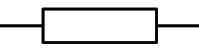
\includegraphics[width=5cm]{weerstand}
\centering
\caption{Symbool van een weerstand}
\label{symbool:weerstand}
\end{figure}


